\chapter{Implementation}
\label{chapter:Chapter 4}
\lhead{Chapter 4. \emph{Implementation}}

In this Chapter, we present a description of the Implementation of \todo[inline]{need a framework name}. Firstly, we provide a Data Analysis from the provided Historical data, which \todo[inline]{needs way more talk}.

\section{Data Analysis}
In order to gain insight and find the limitations of the AIS Data, we decided analyze the provided Historical AIS Data. For this Section, the Data Analysis we used the historical AIS Data-Set made publicly available by \cite{DATASET}.

Analysis of the provided Historical Data, was conducted by firstly analyzing the overall distribution of the Data-Set and after the analysis of each variable. 
The used Data-Set is composed of \textbf{18.684.115} AIS Messages originated by \textbf{4555} different Vessels. The Data-Set covers a Period of 6 Months (from 2015-10-01 to 2016-03-31), from a area nearby Brest, France represented in Figure \ref{fig:DS_Sample}.

\begin{figure}[H]
	\centering
	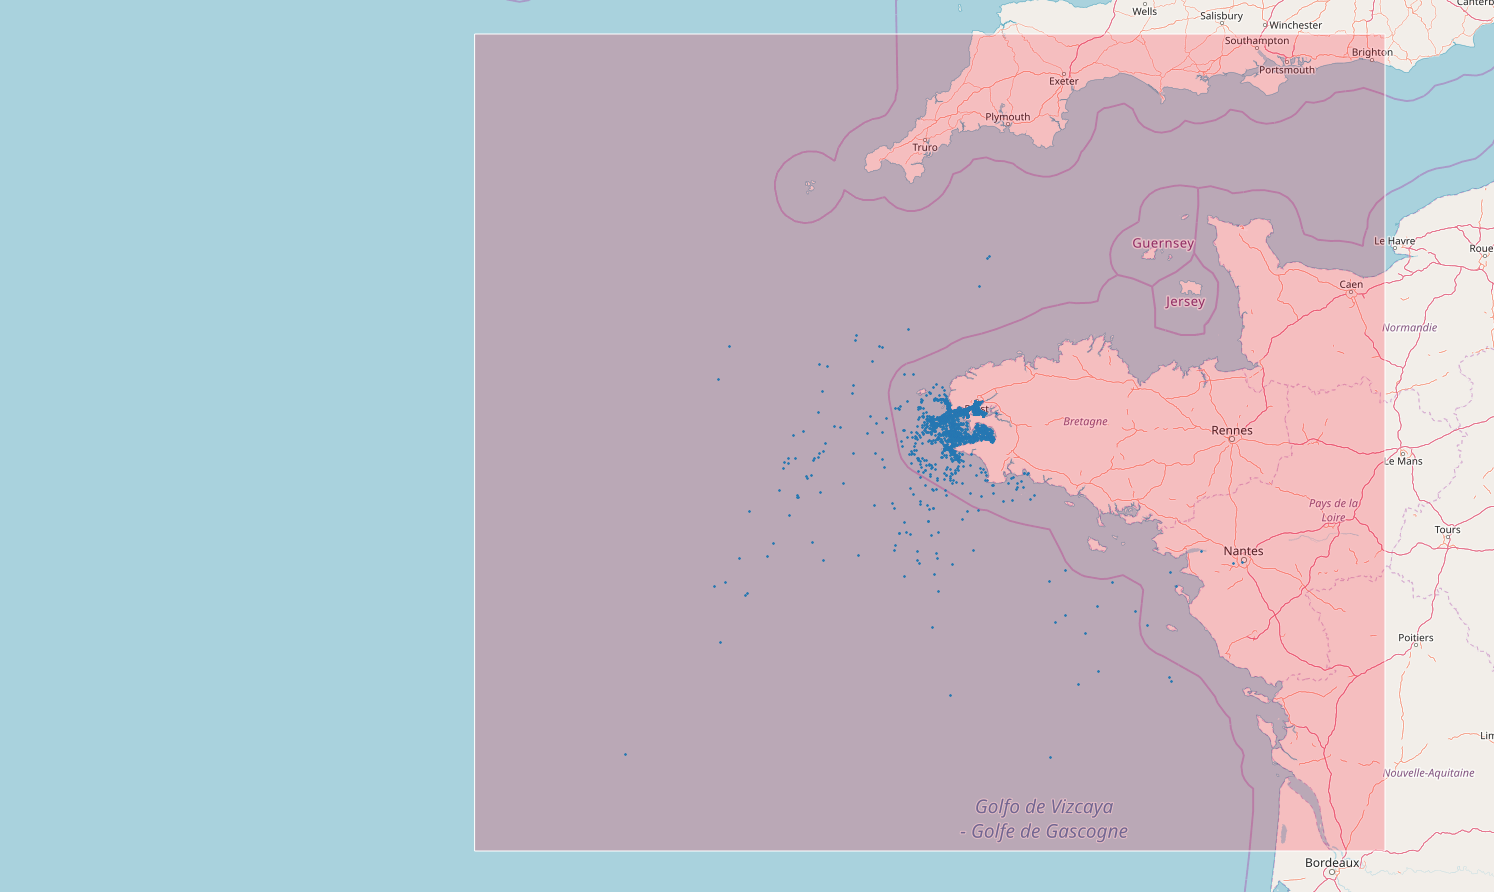
\includegraphics[scale = .23]{figures/Ch4/nari_DS_ex2.png}
    \caption{Area of the Data-Set represented in the Red, with a sample of 50.000 AIS Positions.}
    \label{fig:DS_Sample}
\end{figure}
Which for every  historical AIS Message provided in this Data-Set, contains the following attributes:

\begin{description}
    \item[MMSI] the identifier of the Vessel.
    \item[Status] AIS Navigational Status.  
    \item[Turn] Rate of turn, right or left, 0 to 720 degrees per minute.
    \item[SOG] Speed over ground in knots (allowed values: 0-102.2 knots).
    \item[COG] Course over ground in degrees.
    \item[X] representing the Longitude in degrees.
    \item[Y] latitude in degrees.
    \item[Time] representing the Time-Stamp, of when the message was received.
\end{description}

\todo[inline]{MORE TEXT HERE} The features represented above, were al contained 

\section{Feature Engineering}
\todo[inline]{Needs Intro for this section...} 

\subsection{Latitude Longitude Normalization}
In order to normalize the reported AIS positions, either from the AIS streams or the used Data-Set, we defined a set number of decimal cases used. This is done as most of AIS providers only assure a GPS precision of 0.0001 minutes accuracy, but what we found was that some reported positions come with up to 8 decimal cases, which can be caused just from how the Data-Set files were written.

So our normalization process, was to assure that every Vessel position was normalized to a precision on 4 decimal cases; as it represents a global position precision of 11m to 4m, as it is shown in Table \ref{Table: Degree Precision}.

\begin{table}[H]
\centering
\caption{Degree precision versus the approximate radius of measured error.}
\label{Table: Degree Precision}
\begin{tabular}{lrrrr}
\hline
\multicolumn{1}{c}{\begin{tabular}[c]{@{}c@{}}Decimal \\ Places\end{tabular}} & \multicolumn{1}{c}{Degrees} & \multicolumn{1}{c}{\begin{tabular}[c]{@{}c@{}}Precision \\ Equator\end{tabular}} & \multicolumn{1}{c}{\begin{tabular}[c]{@{}c@{}}Precision \\ 45º N/S\end{tabular}} & \multicolumn{1}{c}{\begin{tabular}[c]{@{}c@{}}Precision \\ 67º N/S\end{tabular}} \\ \hline
0 & 1.0 & 111.3Km & 78.7Km & 43.5Km \\
1 & 0.1 & 11.3Km & 7.8Km & 4.4Km \\
2 & 0.01 & 1.13Km & 787.1m & 435m \\
3 & 0.001 & 111.3m & 78.7m & 43.5m \\
4 & 0.0001 & 11.3m & 7.8m & 4.4m \\
5 & 0.00001 & 1.3m & 0.7m & 0.4m \\ \hline
\end{tabular}
\end{table}

\todo[inline]{Geohash - https://en.wikipedia.org/wiki/Geohash}



\subsection{Distance to Coast}
The Distance to Shore influences, the navigational behaviour for some type of Vessels. In order to enrich the features used in our Anomaly Detection methods it seemed necessary to extrapolate the Distance to Shore for every point in the Data-Set. Although in order to calculate the Distance to Shore over the whole data-set, and in real time to streams of AIS data it is mandatory to represent the Coastline in a efficient manner. 
For this we used the ocean coastline data \todo{insert ref for http://www.naturalearthdata.com}, represented in a vector of \textbf{547.503} points, which is equivalent of representing the coastline with a 1:10m scale.

The calculation of the closest point was done with a Nearest Neighbor approach, using the Ball Tree algorithm. The choice of this algorithm was done, due to the high volume of data we were using, and the possibility of using the Haversine Distance measures \eqref{eq: Haversine} in the already implemented methods from \todo{http://scikit-learn.org/stable/modules/generated/sklearn.neighbors.BallTree.html}.

Haversine is a distance metric commonly used in Vessel Navigation, it is commonly used as both Latitude and Longitude features are represented in a spherical coordinate system. $d$ represents the distance between the 2 point, and $r$ represents the approximate radius of the Earth which for our experiments we used  \textbf{6.367.000m}.
\begin{equation}
d = 2r sin ^{-1} (\sqrt{sin^2(\frac{lat_{2}-lat_{1}}{2})+cos(lat_{1})cos(lat_{2})sin^2(\frac{long_{2}-long_{1}}{2}))}
\label{eq: Haversine}
\end{equation}

\subsection{Stopped/Moving}
Enriching the reported Vessel Kinematics by determining if whether a Vessel is Moving or Stopped represents a information gain on overall Vessel Trajectory that can be addressed, for the understanding of the normal Vessels Behaviour itself and even further, the possible detection of Anomalies.
Thus, the approaches we used to classify every Vessel transmission as Stopped or Moving is shown in the following subsections:

\textbf{Rule Based Approach}:
This approach is vastly used in the literature, as it is the simplest way to characterize the stopping of a Vessel, based solely on the Speed or as reported in the AIS the Speed Over Ground (SOG). Thus, Vessels Positions that have a Speed under a certain defined threshold $\Delta$ are considered as Stopped and the opposite are considered Moving, as it is shown in equation \ref{eq: MovingRule}, where $p_n$ represents actual point we want to the point which we want to c.
\begin{equation}
kinematic status(p_n) = \left\{\begin{matrix}
p_n.SOG > \Delta; & Moving\\ 
p_n.SOG \leq  \Delta; & Stopped
\end{matrix}\right.
\label{eq: MovingRule}
\end{equation}

The most commonly used value, found in the literature for $\Delta$ was 0.5 knots, which was also the Threshold we initially tested for, but we found that this leads to the miss-labeling of effectively Positions that are Moving, more specifically Fishing Vessels that due to their type of fishing activities, greatly slow their Speed for short periods of Time, which cannot be labeled as Stopped.
\todo[inline]{Need intro to this image}
\missingfigure{Trajectory of a Shipping Vessel that is considered as stopped.}

In order to mitigate the problem described above we used a \textbf{Rolling Mean}, which is a common method for Time Series Analysis in countless different fields.  By Smoothing the Vessels Speed Feature, we reduce the random or abrupt variations in the observed Speed features,  thus better describing the normal kinematic, stopping  pattern of a Vessel. 
\todo[inline]{Need intro to this image}
\missingfigure{Trajectory of a Shipping Vessel that is considered as stopped then with the rolling mean!}







\section{TODO}






